\documentclass[a4paper, 11pt, twoside]{article}
\usepackage[utf8]{inputenc}
\usepackage[english, italian]{babel}
\usepackage[a4paper]{geometry}
\geometry{margin=2.5cm}

% Pacchetti
\usepackage{float,graphicx}
\usepackage{hyperref}
% \usepackage[ruled, vlined]{algorithm2e}
% \renewcommand{\thealgocf}{}
\usepackage[T1]{fontenc}
\usepackage{amsmath}
\usepackage{listings}
\usepackage{caption}
\usepackage{xcolor}
\usepackage{siunitx}
\sisetup{
    output-decimal-marker = {,},
    group-separator = {.}
} % Metti numeri grandi nel comando \num{} per usare i corretti separatori di migliaia e virgola
\graphicspath{ {./images/} }
% \linespread{0.9}
\setlength{\parindent}{0cm} % Non indentare nuovi paragrafi
\raggedbottom % Lascia spazio vuoto alla fine della pagina invece di distribuire i paragrafi verticalmente nella pagina, così non ci sono enormi spazi tra i paragrafi

%\DeclareCaptionFont{white}{\color{white}}
%\DeclareCaptionFormat{listing}{\colorbox{gray}{\parbox{\textwidth}{#1#2#3}}}
%\captionsetup[lstlisting]{format=listing,labelfont=white,textfont=white, font=bf}
\lstdefinestyle{codestyle}{
    language=Python,
    breakatwhitespace=false,
    breaklines=true,
    captionpos=b,
    % numbers=left,
    keepspaces=true,
    showspaces=false,
    showstringspaces=false,
    showtabs=false,
    tabsize=2,
    numbersep=5pt,
    columns=fullflexible,
    % frame=lines,
    basicstyle=\ttfamily
}
\newcommand{\horrule}[1]{\rule{\linewidth}{#1}} 
\lstset{style=codestyle}

\title{
    \vspace{-50pt}
    \textsc{Università degli Studi di Udine -- Dipartimento di Scienze Matematiche, Informatiche e Fisiche} \\ 
    \vfill
    \horrule{1pt}\\
    \huge{Relazione 1$^{\circ}$ Progetto del Corso di Social~Computing}\\
    \horrule{1pt}\\
    \vfill
    }
\author{ % In ordine alfabetico (cognome)
    Riccardo Cavasin\\ 
    matr. 144692\\ 
    \vspace{18pt}
    \href{mailto:cavasin.riccardo@spes.uniud.it}{\texttt{cavasin.riccardo@spes.uniud.it}}\\
    Thomas Cimador\\ 
    matr. 152334\\ 
    \vspace{18pt}
    \href{mailto:cimador.thomas@spes.uniud.it}{\texttt{cimador.thomas@spes.uniud.it}}\\
    Alessandro Faion\\ 
    matr. 128378\\ 
    \vspace{18pt}
    \href{mailto:faion.alessandrokenan@spes.uniud.it}{\texttt{faion.alessandrokenan@spes.uniud.it}}\\
}
\date{}

% -------------------------------------------------------------------------------- %
% ------------------------------- INIZIO DOCUMENTO ------------------------------- %
% -------------------------------------------------------------------------------- %
\begin{document}
\begin{titlepage}
    \begin{figure}[t]
        
\includegraphics[width=4.5cm, height=4.5cm]{uniud_logo.png}
        \centering
    \end{figure}
    \maketitle
    \vfill
    \begin{center}
        \large{A.A. 2022-2023}
    \end{center}
    \thispagestyle{empty}
\end{titlepage}

% -------------------------------------------------------------------------------- %
% ------------------------------- INDICE CONTENUTI ------------------------------- %
% -------------------------------------------------------------------------------- %
\tableofcontents
% \listoffigures
% \lstlistoflistings
\thispagestyle{empty}  % Per far cominciare la numerazione delle pagine a partire
\newpage               % dalla pagina successiva (dell'Introduzione)
\setcounter{page}{1}   %

% -------------------------------------------------------------------------------- %
% ------------------------------- INTRODUZIONE ----------------------------------- %
% -------------------------------------------------------------------------------- %
\section{Introduzione}\label{sec:intro}
L'obiettivo di questo primo progetto consiste nel creare ed esaminare una rete di utenti di Twitter.

Si parte da uno specifico account Twitter e si scaricano in cascata gli account che lo seguono (i follower), con una profondità di due livelli (fino ai follower dei follower). Queste informazioni vengono poi utilizzate per costruire due grafi, dei quali se ne analizzano le varie proprietà.

\section{Raccolta e analisi degli account Twitter}
Per poter ottenere dati da Twitter, è richiesto un account developer, che fornisce le chiavi necessarie all'autenticazione delle richieste API REST.

Viene utilizzata la libreria Python Tweepy, che presenta le API di Twitter come metodi dell'oggetto Client:
\begin{itemize}
    \item \texttt{get\_user()}: attributi di default dell'utente richiesto;
    \item \texttt{get\_users\_followers()}: i follower dell'utente;
    \item \texttt{search\_recent\_tweets()}: query sui tweet più recenti; in questo caso vengono scaricati i tweet dell'ultima settimana;
\end{itemize}

L'account ``radice'' di partenza è \texttt{@KevinRoitero}. Degli account follower di questo utente vengono scaricati:
\begin{itemize}
    \item Gli attributi di default (ID dell'account, nome del profilo, nome utente);
    \item La descrizione del profilo;
    \item Le metriche pubbliche dell'account (numero di follower, numero di following, numero di tweet, numero di liste in cui appare l'account);
    \item Se l'account risulta protetto (i suoi tweet sono disponibili soltanto ai followers);
\end{itemize}

Tutte queste informazioni vengono infine serializzate su un file in formato JSON con chiave l'ID.

\section{Creazione della rete sociale}
Utilizzando la libreria NetworkX, viene costruito un \textit{grafo diretto}, dove:
\begin{itemize}
    \item Ogni nodo corrisponde ad un utente Twitter, limitandosi all'utente radice e i suoi follower diretti;
    \item L'ID del nodo è uguale all'ID utente;
    \item Ciascun nodo ha come attributi:
          \begin{itemize}
              \item L'username
              \item La descrizione
              \item Il numero di follower del profilo corrispondente
          \end{itemize}
    \item Gli archi (collegamenti) corrispondono alle relazioni di following (un utente che segue un altro).

          Se due utenti si seguono a vicenda, saranno due nodi collegati da due archi di verso opposto.
\end{itemize}

Viene anche costruito un \textit{grafo indiretto} a partire dal primo, al quale vengono aggiunti altrettanti nodi casuali con il metodo dell'attaccamento preferenziale (Preferential Attachment).

Qui vengono mostrate visualizzazioni dei grafi generate con NetworkX, usando il layout di Fruchterman-Reingold.\\
È anche possibile generarne una visualizzazione HTML interattiva mediante la libreria PyVis.

\begin{figure}[H]
    \centering
    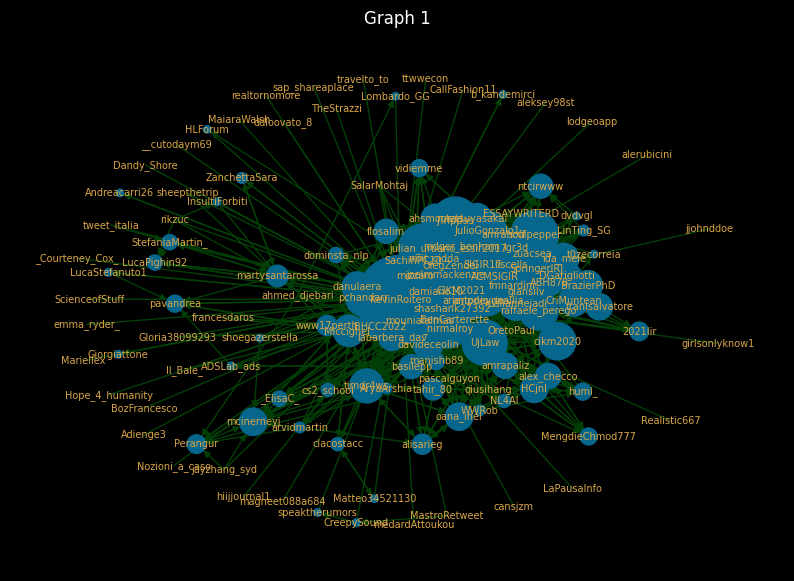
\includegraphics[width=.45\textwidth, keepaspectratio]{directed_graph.png}
    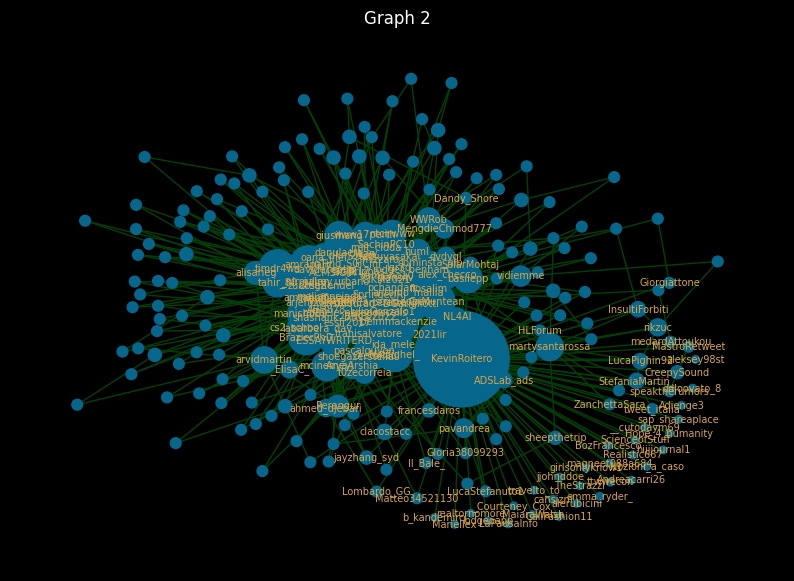
\includegraphics[width=.45\textwidth, keepaspectratio]{non_directed_graph.png}

    Grafo diretto (sinistra) e grafo indiretto (destra)
\end{figure}

\section{Analisi della rete}
Una volta creati i grafi, si può usare la libreria NetworkX anche per effettuare varie misurazioni ed analizzarne le loro proprietà.

In questo documento, si userà il termine \textit{cammino} per indicare il cammino minimo tra due nodi in un grafo.

\subsection{Componente fortemente connessa}
In un grafo è possibile identificare una componente connessa \textit{CC}, ovvero un sottografo connesso. In un grafo diretto, una componente si dice fortemente connessa \textit{SCC} se per ogni coppia di nodi esiste un cammino che li collega.

Per come è stato costruito il grafo indiretto, è garantita l'assenza di nodi sconnessi, quindi, la rispettiva CC corrisponde all'intero grafo.

\subsection{Misurazioni}
Sono state studiate varie metriche basate sui cammini:

\subsubsection{Raggio}
Il raggio è uguale all'eccentricità minima. L'eccentricità di un nodo è la massima lunghezza tra tutti i cammini da tale nodo agli altri nodi nel grafo. Per definizione, l'eccentricità può essere calcolata solo se ogni nodo è raggiungibile da ogni altro nodo. Nel caso dei grafi diretti, bisogna limitarsi ad una SCC.
\begin{itemize}
    \item Nel caso del grafo diretto, il raggio della SCC risulta 3. Non esiste un nodo adiacente a tutti gli altri.
    \item Nel caso del grafo indiretto, il raggio della CC risulta 2. L'assenza di direzionalità ha creato nuovi cammini più brevi. La lunghezza dei cammini era limitata dalla direzione degli archi. I nodi aggiuntivi non hanno influenzato negativamente questo parametro.
\end{itemize}

\subsubsection{Centro}
Il centro è l'insieme dei nodi con eccentricità minima, ovvero uguale al raggio.
\begin{itemize}
    \item Nel caso del grafo diretto, il centro della SCC è composto dagli utenti:
          \begin{lstlisting}
['KevinRoitero', 'davideceolin', 'joelmmackenzie', 'labarbera_dav', 'BHCC2022', '_nirmalroy', 'timdr4ws', 'CIKM2021', 'rmit_cidda', 'damiano10', 'Miccighel_']\end{lstlisting}
          Questi utenti sono connessi agli altri nodi in maniera analoga a \texttt{@KevinRoitero}, e si possono considerare utenti ``radice'' allo stesso modo.
          Un'altra osservazione interessante è che \texttt{@KevinRoitero} è seguito a sua volta dagli altri utenti ad un livello tale da essere incluso nel centro.
    \item Nel caso del grafo indiretto, il centro della CC è \texttt{@KevinRoitero}. Ciò vuol dire che l'unico utente la cui eccentricità dipende dalla direzionalità degli archi. Questo è verosimile, perché tutti gli archi entranti di \texttt{@KevinRoitero} ora possono essere percorsi in uscita.
\end{itemize}

\subsubsection{Distanza media tra i nodi (diametro)}
Questa metrica indica la lunghezza media di tutti i cammini nel grafo.
\begin{itemize}
    \item Nel caso del grafo diretto, il cammino medio nella SCC è lungo 2.00. Questo deriva probabilmente dal numero di livelli che avrebbe idealmente l'albero dei followers senza cicli, e la numerosità delle foglie domina la media.
    \item Nel caso del grafo indiretto, il cammino medio nella CC è lungo 2.54. Questo suggerisce che i nodi aggiunti con il Preferential Attachment, possedendo solo due archi uscenti, tendano ad assumere un ruolo ``periferico'', allungando di un arco i cammini associati.
\end{itemize}

Si osserva inoltre che il diametro del grafo diretto non è limitato dalla direzione degli archi, perché
la non-direzionalità non ha diminuito osservabilmente la lunghezza dei cammini medi.

\subsubsection{Distanza massima tra due nodi}
Questa metrica indica la lunghezza massima di tutti i cammini nel grafo.
\begin{itemize}
    \item Nel caso del grafo diretto, il cammino massimo nella SCC è lungo 4. Questo deriva probabilmente dal cammino massimo in un albero di due livelli (da foglia sinistra a foglia destra).
    \item Nel caso del grafo indiretto, il cammino massimo nella CC è lungo 4. Ciò sostiene quanto detto nell'osservazione precedente.
\end{itemize}

\subsection{Centralità}
Sono state studiate alcune metriche che misurano varie proprietà di ciascun nodo nel grafo:

\subsubsection{Betweenness}
La betweenness misura quanto un nodo è importante nel connettere altri nodi. Si enumerano tutti i cammini nel grafo e si controlla quale nodo appare più spesso. In formula:

$$
    c_B(v)=\sum_{s,t\in V}\frac{\sigma(s,t\mid v)}{\sigma(s,t)}
$$

Dove $V$ è l'insieme dei nodi, $\sigma(s,t)$ è il numero di cammini tra $(s,t)$, e $\sigma(s,t\mid v)$ è il numero di cammini che attraversano il nodo $v$ eccetto quelli tra $s,t$.

\begin{itemize}
    \item Nel caso del grafo diretto, il nodo con la betweenness maggiore è l'utente \texttt{@KevinRoitero}, di un ampio margine. Essendo l'utente radice, questo è ragionevole.
    \item Nel caso del grafo indiretto, la situazione è analoga. La non-direzionalità e il Preferential Attachment non hanno influenzato la distribuzione della betweenness.
\end{itemize}

\subsubsection{Closeness}
Centralità di vicinanza, ovvero quanto più velocemente un nodo è raggiunto dagli altri nodi.

$$
    C(u)=\frac{n-1}{\sum_{v=1}^{n-1}d(v,u)}
$$

Dove $d(v,u)$ è la lunghezza del cammino da $v$ a $u$, e $n-1$ è il numero di nodi raggiungibili da $u$ (è l'inverso di una media).

\begin{itemize}
    \item Nel caso del grafo diretto, il nodo con la closeness maggiore è l'utente \texttt{@KevinRoitero}, in questo caso, la distribuzione è più uniforme. Più della metà degli altri nodi presentano valori di closeness vicini alla mediana.
    \item Nel caso del grafo indiretto, esistono più nodi con closeness bassa.
\end{itemize}

\subsubsection{Degree}
Centralità di grado, ovvero la frazione dei nodi adiacenti al nodo. La centralità di grado indica quanto un nodo è ``al centro'' del grafo.

$$
    C_{d}(v_i)=\frac{d_i}{n-1}
$$

Dove $v_i$ è il grado del nodo $v_i$, e $n-1$ è il massimo grado possibile per $n$ nodi connessi.

Può essere calcolata per archi indiretti, (centralità Degree), per archi in entrata (centralità In-Degree), o per archi in uscita (centralità Out-Degree).

Nel caso del grafo diretto:
\begin{itemize}
    \item Il nodo con la centralità In-Degree maggiore è l'account \texttt{@KevinRoitero}. Pochi altri nodi hanno valori vicini alla mediana, e tutti gli altri hanno valori sotto la mediana.
    \item Il nodo con la centralità Out-Degree maggiore è sempre l'account \texttt{@KevinRoitero}. Un solo nodo ha un valore particolarmente vicino ad esso. Circa metà degli altri nodi presentano valori intorno alla mediana, e i nodi ``periferici'' hanno valori bassi.
\end{itemize}
Nel caso del grafo indiretto, il nodo con la centralità degree maggiore è l'account \texttt{@KevinRoitero}, ed è visibile un piccolo gruppo di nodi con valori vicini alla mediana.

\subsubsection{PageRank}
PageRank è una centralità ricorsiva, dove ogni nodo ha un valore PageRank inizialmente calcolato in base ai suoi collegamenti in entrata. Per ogni nodo, tale valore aumenta se questo ha collegamenti in ingresso da altri nodi con alto PageRank.

\begin{itemize}
    \item Nel caso del grafo diretto, il nodo con il valore PageRank maggiore è l'utente \texttt{@KevinRoitero}.
    \item Nel caso del grafo indiretto, il nodo con il valore PageRank maggiore è sempre l'utente \texttt{@KevinRoitero}, mentre il resto dei nodi presenta un valore decisamente più basso.
\end{itemize}

\subsubsection{HITS}
La centralità HITS (Hyperlink-Induced Topic Search) classifica i nodi in base a due valori, Hub e Authority. Il valore Hub di un nodo stima il valore delle sue relazioni con gli altri nodi, in base ai suoi archi uscenti. Il valore Authority stima l'importanza del nodo all'interno della rete, in base ai suoi archi entranti.

\begin{itemize}
    \item Nel caso del grafo diretto, la maggioranza dei nodi sono Hub e hanno pochi o nessun arco in uscita.
    \item Nel caso del grafo indiretto, si verifica una distribuzione abbastanza equa di Hub e Authority.
\end{itemize}
Il nodo \texttt{@KevinRoitero} è un'Authority in entrambi i grafi.

\subsection{Small World-ness}
Vengono calcolati i coefficienti Omega ($\omega$) e Sigma ($\sigma$) per determinare l'effetto piccolo mondo (Small World-ness), ovvero se il grafo ha una distanza piccola e un clustering alto. Un coefficiente di clustering alto indica che i vicini di un certo nodo tendono ad essere a loro volta vicini tra di loro.

I due coefficienti sono definiti:

$$
    \omega = \frac{L_r}{L} - \frac{C}{C_l}
$$
$$
    \sigma = \frac{C}{Cr} / \frac{L}{L_r}
$$

Dove $L$ è il cammino medio del grafo, $C$ è il coefficiente di clustering medio, e $L_r$ e $C_r$ sono gli stessi valori per un grafo casuale equivalente. $C_l$ è il coefficiente di clustering medio per un grafo regolare equivalente.

Tali coefficienti sono definiti solo per i grafi indiretti, quindi per il primo grafo viene utilizzata una vista indiretta.

\begin{itemize}
    \item Nel caso del grafo diretto, il coefficiente $\omega$ è circa 0.097 e il coefficiente $\sigma$ è circa 1.234.
    \item Nel caso del grafo indiretto, il coefficiente $\omega$ è circa 0.146 e il coefficiente $\sigma$ è circa 1.345.
\end{itemize}

Il valore di $\omega$ è vicino a 0 se una rete ha proprietà small-world. Secondo questo parametro, entrambi i grafi possono essere considerati small-world.

Il valore di $\sigma$ è $>1$ se una rete ha proprietà small-world. Secondo questo parametro, entrambi i grafi possono essere considerati small-world.

Entrambi i grafi modellano una rete sociale esistente, quindi i risultati sono giustificati. In più, si osserva che la tecnica del Preferential Attachment ha conservato correttamente la proprietà di small-world-ness.

\end{document}
